\section{App 介绍}

\subsection{背景}

艺术是人们生活中必不可少的事物。近些年来随着移动媒体技术的发展,人们可以很方便地在自己的移动设备上拍摄照片或者倾听音乐,进行艺术的欣赏。但是对于大多数人来说,艺术创造距离他们似乎比较遥远。我们相信许多人一定曾经畅想下面这样的场景:
,

\textbf{随手拍的一张图片可以拥有与梵高的《星夜》相同的艺术风格,即兴演奏的小提琴曲可以拥有钢琴的音色,或者,使用周杰伦的歌声去翻唱陈奕迅的《十年》,想想都很有趣吧!}当今AI的快速发展为这些看起来不可能实现的事情提供了可能。

本App的设计初衷就是希望通过现在飞速发展的AI技术来让每一个普通人都有创造属于自己的艺术作品的机会,借助前辈们的作品来进行二次制作,探索不同的艺术风格以激发自己的创造灵感,满足自己的艺术欣赏需求。同时本app还设计了一体化的社区和探索模块,在欣赏前辈艺术家作品和二创作品的同时,还可在共享社区中找到志趣相近的朋友。

\subsection{开发进度}

App 的两大核心功能——音乐艺术加工以及图像艺术加工,均有训练效果较好的神经网络模型部署在后端服务器上,同时 App 的社区功能也较完善,用户可以发布或收藏他人的作品。前端 UI 基本设计完毕,同时完成了核心功能的后端 API 以及所需数据库构建。\textbf{本 App 的所有设计开发工作均在正式比赛期间进行},由于开发时间较短,网络通信模块的部分功能暂未实现,未来会进一步开发和完善。

\subsection{部分功能介绍}

\subsubsection{图像艺术加工}

图像是艺术的一个重要载体。人们日常生活中会拍摄大量的照片,当前很多社交软件上用户也可分享自己拍摄的照片。本App提供的图像艺术加工功能可以使用户拍摄的图片进行艺术风格化。用户在提供内容图片(本机所拍摄图片)和目标风格图片后,会获得风格化后的原内容图像,具体交互步骤参考展示视频。

\begin{figure}[H]
    \centering
    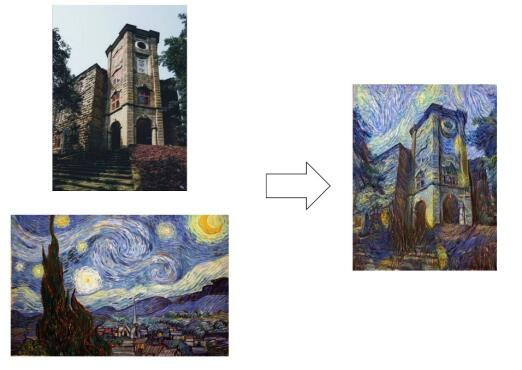
\includegraphics[width=0.8
    \textwidth]{figures/img-trans.jpg}
    \caption{图像加工示意图}
    \label{fig:my_label}
\end{figure}

\subsubsection{音乐艺术加工}

如何让自己喜欢的歌手去翻唱另外一个歌手的音乐呢?在现实中,这是较难实现的。然而,借助神经网络我们可以实现\textbf{音色风格的迁移},这也是本 App 的核心创新点。

用户首先选定需要转化的音乐,之后选择喜爱歌手的音色,\textbf{本 App 后端服务器部署了音乐风格迁移模型并存储了开源的部分歌手音色数据,首先对原始音乐文件进行数据格式转换等预处理操作转化为模型所需的数据,之后进行模型的训练,最终输出转换后的音乐}。

不仅如此,本 App 还提供了\textbf{音乐风格转换功能},让你的口哨变为莫扎特风!或者将喜欢的钢琴曲转为小提琴曲而安利给你的朋友!

\subsubsection{社区}

社区是交友类/社交类 App 的常见功能模块。因为本 App 的设计初衷之一就希望用户能够在社区分享自己的作品并且以此为契机找到志趣相近的好友,所以设计并实现了社区这一功能模块。用户能够在社区发帖,上传自己制作的图片或者音频,也可以欣赏他人的作品并进行评论或者收藏。具体界面如下图所示:

\begin{figure}[H]
    \centering
    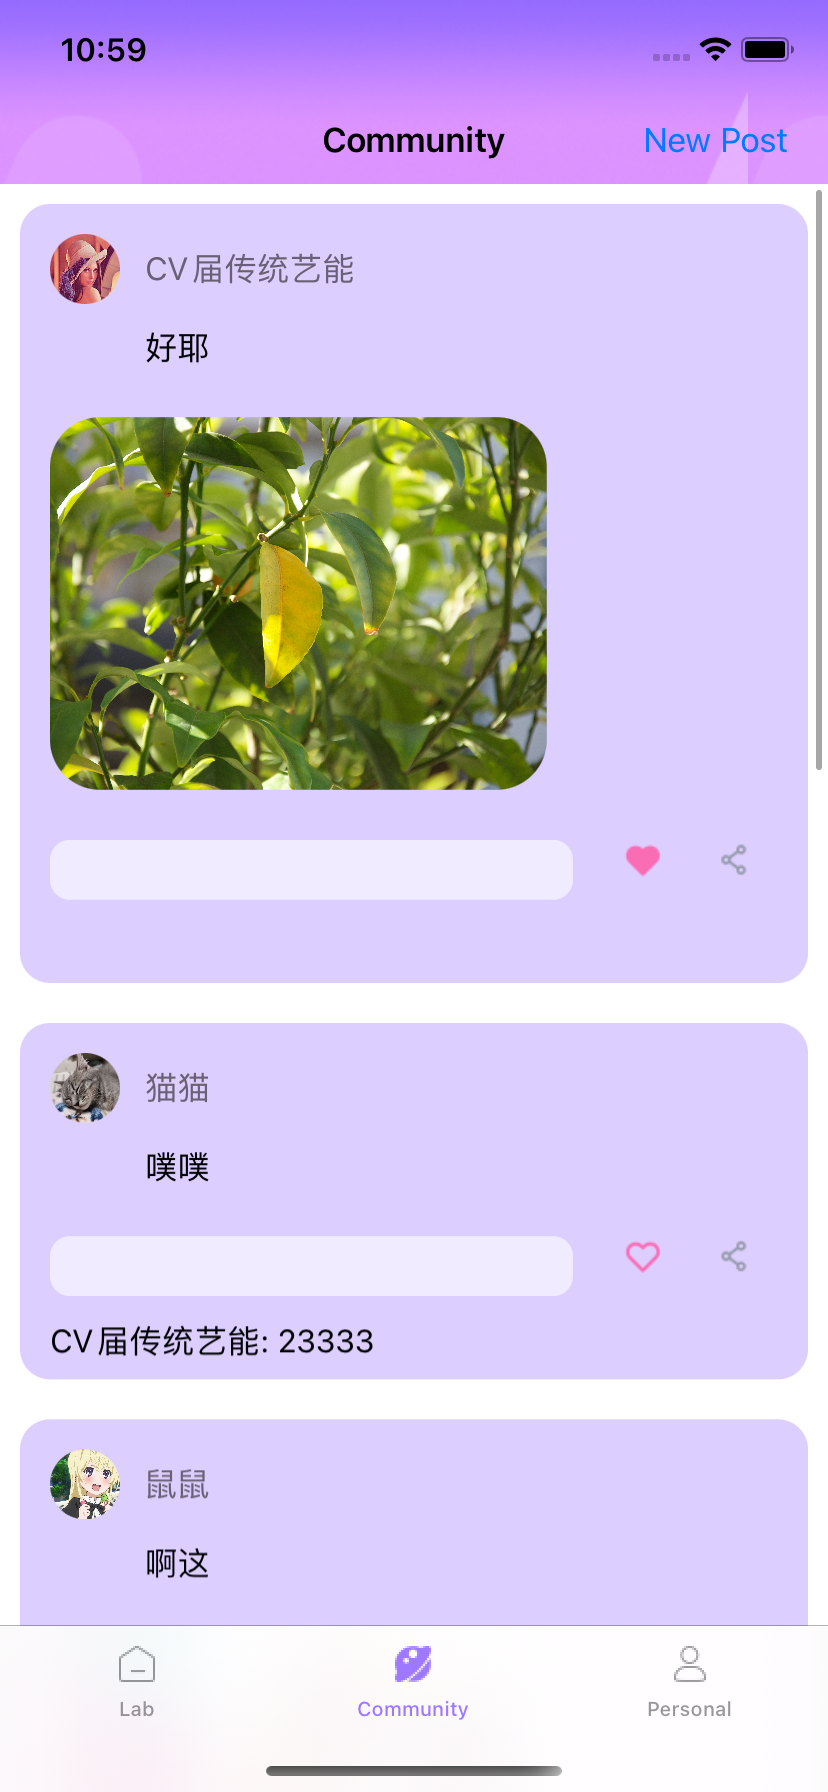
\includegraphics[width=0.5
    \textwidth]{figures/社区.png}
    \caption{社区示意图}
    \label{fig:my_label}
\end{figure}

\subsection{用户信息}

本 App 后端数据库存储了不同用户的信息,如收藏和创作的帖子、账户密码等,这可以方便用户快捷的进行操作,如修改个人信息、寻找历史浏览记录等。针对登录功能,为了保证用户密码的安全性,防止网络传输过程中被他人窃取,\textbf{本 App 采用HMAC 加密算法来对用户密码信息进行加密,提高了安全性。}
